%\subsection{多源迁移学习 (multi-source TL)}

\begin{frame}
    \frametitle{迁移学习:多源迁移学习}
    \begin{itemize}
        \item 多源迁移学习
            \begin{itemize}
                \item 问题定义:多个源域和目标域,如何进行有效的域筛选,从而进行迁移?
            \end{itemize}
        \item 代表方法
            \begin{itemize}
                \item TrAdaBoost [Dai, ICML-07]
                \item MsTL-MvAdaboost [Xu, ICONIP-12]
                \item Consensus regularization [Luo, CIKM-08]
                \item Transitive transfer learning [Tan, KDD-15]
                \item Distant domain TL [Tan, AAAI-17]
            \end{itemize}
    \end{itemize}
\end{frame}

\begin{frame}
    \frametitle{迁移学习:多源迁移学习}
    \begin{itemize}
        \item TrAdaBoost [Dai, ICML-07]
            \begin{itemize}
                \item 利用Boost的技术过滤掉多个源域中与目标域不相似的样本,然后进行实例迁移学习
            \end{itemize}
    \end{itemize}
    \begin{figure}
        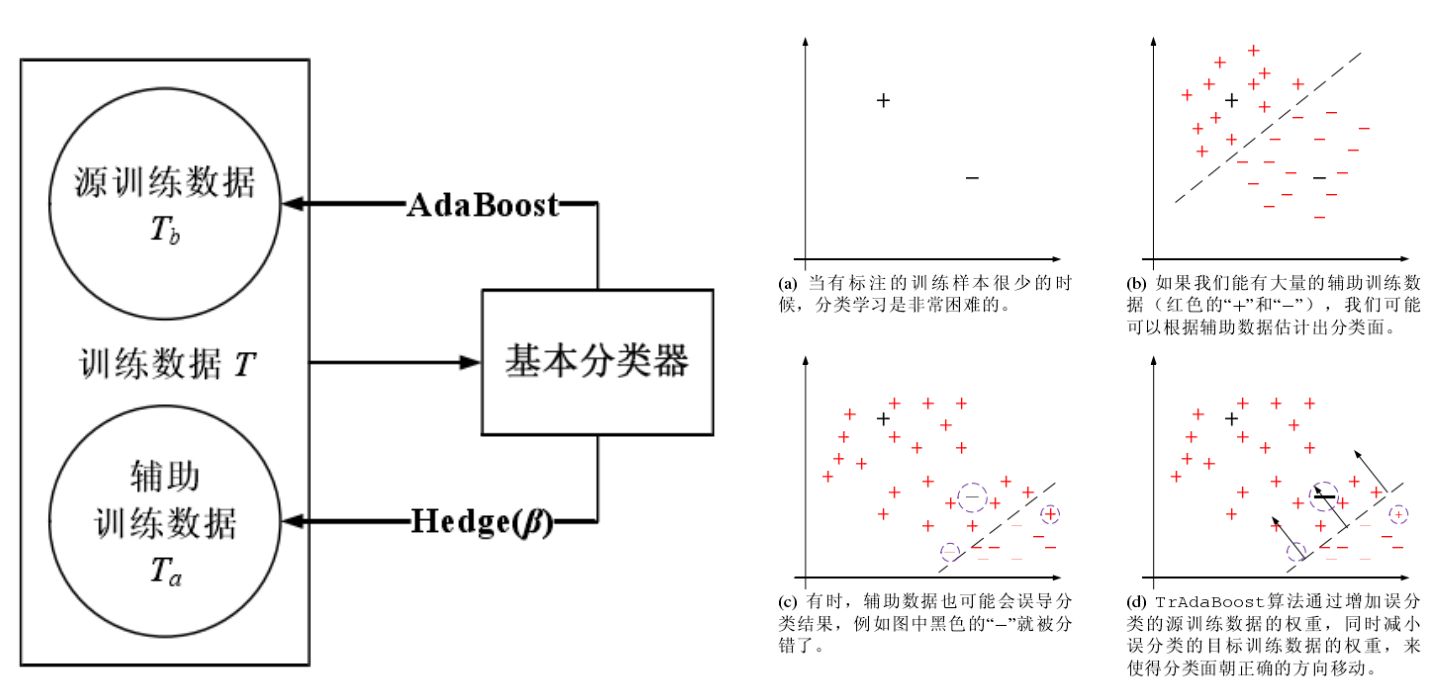
\includegraphics[width=0.9\textwidth]{tradaboost.png}
    \end{figure}
\end{frame}

\begin{frame}
    \frametitle{迁移学习:多源迁移学习}
    \begin{itemize}
        \item MsTL-MvAdaboost [Xu, ICONIP-12]
            \begin{itemize}
                \item 不仅考虑源域和目标域的样本相似度情况,同时以多视图学习的目标来进行统一的迁移
            \end{itemize}
        \item Consensus regularization [Luo, CIKM-08]
            \begin{itemize}
                \item 同时在源域和伪标注的目标域上训练分类器,利用一致性约束进行知识的迁移
            \end{itemize}
    \end{itemize}
\end{frame}

\begin{frame}
    \frametitle{迁移学习:多源迁移学习}
    \begin{itemize}
        \item Transitive transfer learning [Tan, KDD-15]
            \begin{itemize}
                \item 在两个相似度不高的域中,利用从第三方中学习到的相似度
                关系,完成知识的传递迁移
            \end{itemize}
    \end{itemize}
    \begin{figure}
        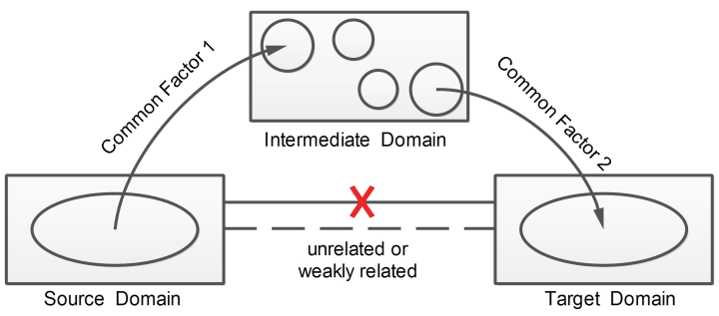
\includegraphics[width=0.9\textwidth]{ttl.jpg}
    \end{figure}
\end{frame}

\begin{frame}
    \frametitle{迁移学习:多源迁移学习}
    \begin{itemize}
        \item Distant domain TL [Tan, AAAI-17]
            \begin{itemize}
                \item 在相似度极低的两个域进行迁移时,用autoencoder自动从
                多个中间辅助域中选择知识,完成迁移
            \end{itemize}
    \end{itemize}
    \begin{figure}
        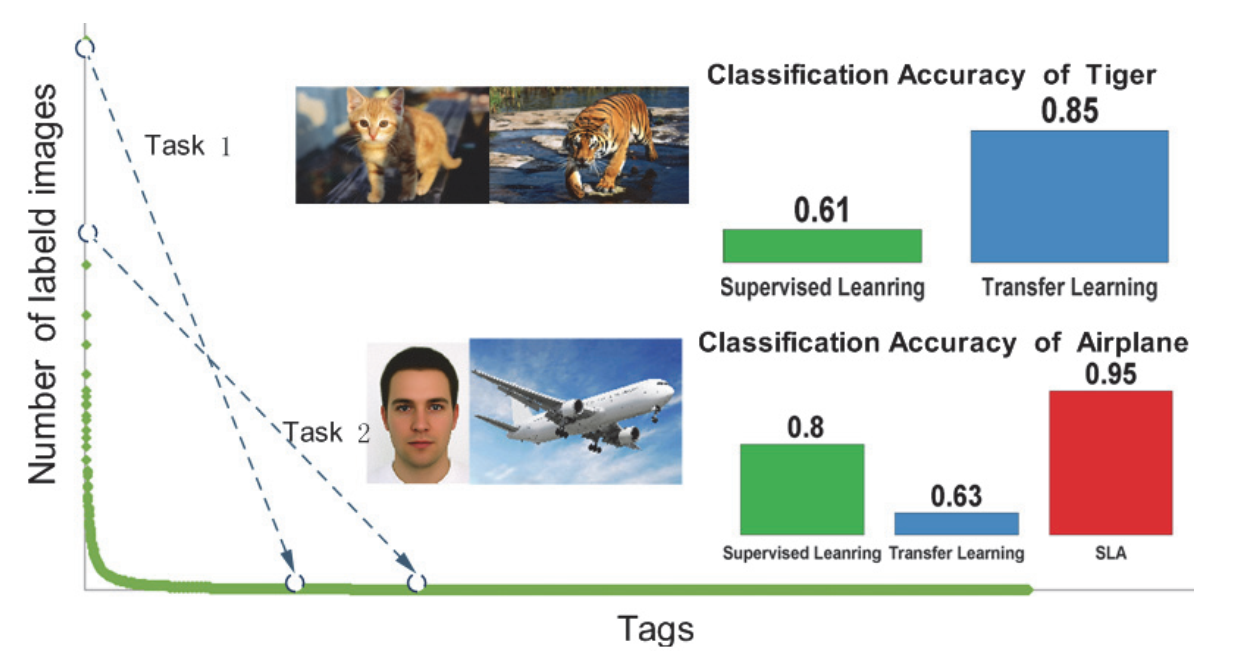
\includegraphics[width=0.9\textwidth]{sla.png}
    \end{figure}
\end{frame}

\begin{frame}
    \frametitle{迁移学习:多源迁移学习}
    \begin{itemize}
        \item 总结
        \begin{itemize}
            \item 多源迁移学习可以有效利用存在的多个可用域,综合起来进
            行迁移,达到较好的效果
            \item 如何衡量多个域之间的相关性还是一个问题
            \item 对多个域的利用方法也存在一定挑战性
        \end{itemize}
    \end{itemize}
\end{frame}